\chapter{\label{chapter5}Discussion}

In this chapter we will discuss the convergence times of iSDX with and without Swift in \ref{chapter5:Convergence time}. We will evaluate the VMAC partitioning in \ref{chapter5:vmac evaluation} and examine the fast reroute flow rules in \ref{chapter5:number of flow rules}

\section{\label{chapter5:Convergence time}Convergence time}

\rb{discuss results and overhead and swift performance}

\section{\label{chapter5:vmac evaluation}VMAC Evaluation}

Since both the iSDX and Swift use the destination mac address to encode different information, the amount of bits available to  the iSDX and Swift is reduced. The current VMAC partitioning is simply the first intuition on how the VMAC can be partitioned. The partitioning can be easily changed by configuring the iSDXs parameters. There may still be some optimization. But we realize that optimizing the VMAC partitioning would outgrow the time frame of this project. In this section we evaluate the VMAC partitioning in its current state.

\begin{figure}[h]
\center
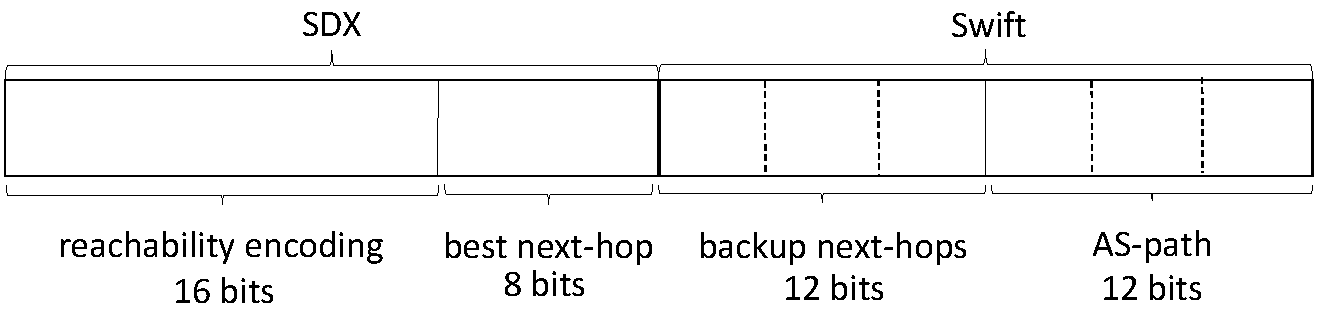
\includegraphics[scale = 0.65]{Figures/eval_vmac_cropped2.pdf}
\caption{Vmac of the iSDX with Swift}
\end{figure}

In its current state 24 bits are allocated to the iSDX. 16 bits for the reachability encoding and 8 bits for the BGP best next-hop. \\
The amount of bits allocated for the best next-hop limits the number of participants the iSDX with Swift can have. The number of participants is limited to $2^8$ = 256. \\
24 bits are allocated to Swift. 12 bits are used to encode backup next-hops and 12 bits are used for the AS-path encoding. \\
With 12 bits used for the AS-path encoding the encoding has a coverage performance of about 85\%. (see Swift paper Figure 9)\\
12 bits for 3 backup next-hops means 4 bits for each next-hop. This means that every participant can have 16 backup next-hops at most. This is not a lot and after 16 backup next-hops have been assigned some prefixes will end up with no backup next-hop. On the other hand it also limits the number of fast reroute rules. \\


\section{\label{chapter5:number of flow rules}Fast Reroute Flow Rules}

In this section we will first examine the number of Fast reroute Flow Rules required for a Fast-Reroute in \ref{chapter5:number of flow rules:number_of_Flow_Rules}. We will also examine the priority of the Fast-Reroute Flow Rules compared to Outbound Policies in \ref{chapter5:number of flow rules:outbound_FR}

\subsection{\label{chapter5:number of flow rules:number_of_Flow_Rules}Number of Flow Rules}

After a Fast Reroute message has been received the FR handler pushes Fast Reroute rules into the IXP fabric. For every backup next-hop that the participant has stored a rule is pushed. This means the maximum number of rules pushed by a participant after a Fast Reroute is 16. \\
FR messages get sent to every participant that is peering with the participant whose Swift-BPA triggered the Fast Reroute. This means the maximum number of flow rules pushed after a Fast Reroute is triggered is 256*16 = 4096. This amount of flow rules is not substantial enough to have a significant impact on the iSDX. With the number of participants limited to 256 and participants having a reasonbale number policies, the flow rule limit for current SDN switches should not be reached. (iSDX paper figure 3 (a) amsix paper figure 9 )\\
Usually this upper bound of flow rules should not be reached. Upon a Fast-Reroute not all participants will be peering with the participant that triggered the Fast Reroute. Also the participants may not have reached the maximum number of Flow Rules yet.

\subsection{\label{chapter5:number of flow rules:outbound_FR}Outbound Policies and Fast Reroute Rules}

Fast Reroute rules and Outbound Policies are in conflict.\\
If Outbound policies have a higher priority than Fast Reroute rules, packets that match the policy may be rerouted to a backup next-hop or they may be rerouted to a participant whose BGP route traverses the failed AS-link. \\
If Fast Reroute rules have a higher priority then the participants Outbound policies will be ignored. \\
Due to the limited number of bits available, encoding the AS-path and backup next-hops of the participants routes in the reachability encoding is not feasible. In the current iSDX with Swift Fast Reroute rules have a higher priority than Outbound policies. Future work may allow participants to define which Outbound policies they want overridden by Swift and which ones not. But this goes beyond the scope of this project.

